\documentclass[border=4pt]{standalone}
\usepackage{tikz}
\usetikzlibrary{arrows,arrows.spaced,positioning}
\begin{document}
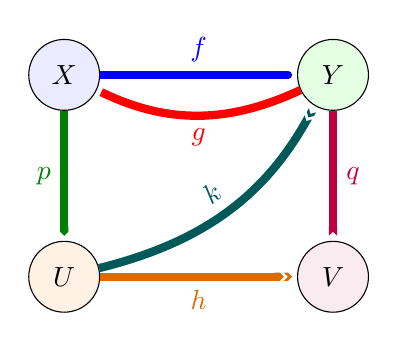
\begin{tikzpicture}[
  node distance=1.65cm and 2.5cm,
  obj/.style={draw,circle,minimum size=9mm,inner sep=1pt}
]
  \node[obj,fill=blue!8] (X) {$X$};
  \node[obj,fill=green!10,right=of X] (Y) {$Y$};
  \node[obj,fill=orange!10,below=of X] (U) {$U$};
  \node[obj,fill=purple!8,right=of U] (V) {$V$};

  \draw[blue,line width=3pt,-{spaced round cap}] (X) -- node[above] {$f$} (Y);
  \draw[red,line width=3pt,-{spaced butt cap}] (Y) to[bend left=25] node[below] {$g$} (X);
  \draw[green!50!black,line width=3pt,-{spaced triangle 90 cap}] (X) -- node[left] {$p$} (U);
  \draw[purple,line width=3pt,-{spaced triangle 90 cap reversed}] (Y) -- node[right] {$q$} (V);
  \draw[orange!85!black,line width=3pt,-{spaced fast cap}] (U) -- node[below] {$h$} (V);
  \draw[teal!70!black,line width=3pt,-{spaced fast cap reversed}] (U) to[bend right=23] node[above,sloped] {$k$} (Y);
\end{tikzpicture}
\end{document}
